\documentclass[12pt]{article}
\usepackage[utf8]{inputenc}
\usepackage{graphicx}
\usepackage{hyperref}
\hypersetup{
    colorlinks=true,
    linkcolor=blue,
    urlcolor=magenta,
}
\graphicspath{ {./images/} }

\title{Rapport stage}
\author{Max Cohen}
\date{September 2020}

\begin{document}

\begin{titlepage}
    \maketitle
\end{titlepage}

\tableofcontents

\section{Introduction}

\subsection{Context}
In 2009, the buidling industry accounted for over 40\% (see \ref{consumption_repartition}) of the total French energy consumption, as well as almost a quarter of greenhouse emissions (Loi Grenelle\footnote{\href{https://www.legifrance.gouv.fr/loda/id/JORFTEXT000020949548/2020-09-21/}{Loi Grenelle I, Article 3}}). In the ecological context where energy waste can no longer be ignored, bridging the energy efficiency gap of the buidling industry would be the first step in reducing the State impact on the environnement\footnote{\href{http://temis.documentation.developpement-durable.gouv.fr/docs/Temis/0067/Temis-0067836/18854.pdf}{Plan d'action national en faveur des énergies renouvelables}}. This translated as a 38\% reduction objective in the consumption of the building industry for 2020\footnote{\href{https://www.legifrance.gouv.fr/loda/id/JORFTEXT000020949548/2020-09-21/}{Loi Grenelle I, Article 5}}, through the renovation of 400 000 apartments per year.

\begin{figure}
    \caption{French consumption repartition (\href{https://www.ecologie.gouv.fr/action-france-lefficacite-energetique}{Action de la France pour l’efficacité énergétique})}
    \centering
    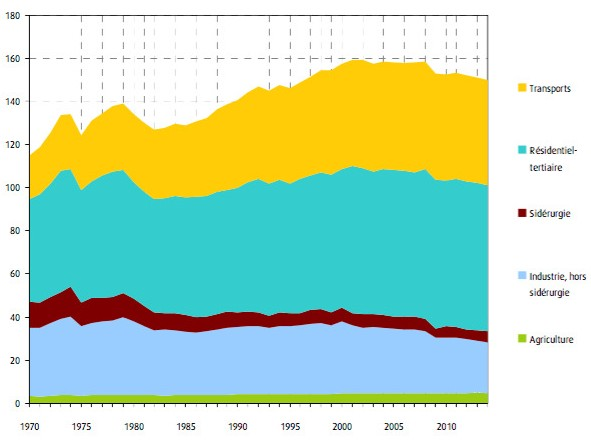
\includegraphics[width=0.8\textwidth]{consumption_evolution_1970_2015.jpg}
    \label{consumption_repartition}
\end{figure}

Amid the anticipation of the Paris Aggreement, that would eventually require from each endorsing country to communicate their own yearly greenhouse emissions\footnote{\href{https://unfccc.int/files/meetings/paris_nov_2015/application/pdf/paris_agreement_english_.pdf}{Paris Agreement}}, the government issued a new law regarding the ecological transition: the LTECV. It's contribution toward building energy efficiency mainly revolves around improving and speeding up the renovation effort, raising the previous objective to 500 000 apartments per year\footnote{\href{https://www.legifrance.gouv.fr/jorf/id/JORFTEXT000031044385/}{Loi relative à la Transition Energétique pour la Croissance Verte, Article 3}}.

However, depsite setting higher and higher objectives toward renovating the French buidling park, the government still falls short in terms of results, as stated by the Ademe (Agency for the environnement and energy)\footnote{\href{https://www.lefigaro.fr/conjoncture/accord-de-paris-pourquoi-les-pays-ne-sont-pas-a-la-hauteur-de-leurs-engagements-20190419}{Hervé Lefebvre, head of the Climat departiement of the Ademe, 2019}}. According to the National Low-Carbon Strategy (SNBC), the average number of yearly renovation only reaches 370 000 for the period 2015-2030\footnote{\href{https://www.ecologie.gouv.fr/strategie-nationale-bas-carbone-snbc}{Stratégie Nationale Bas-Carbone (SNBC)}}.

\subsection{Oze-Energies}

Oze-Energies is a French company specialized in real estate management. Through innovative and durable methods, it aims at improving air quality and confort, while simultaneous reducing energy consumption, without requiring any site work.

The premise of buidling management at Oze is the ability to produce tailored roadmap for managing a building, based on a precise understanding of its behavior, combined with prior knowledge in thermal physics as well as meteo forcasts. While environnemental sensors are integrated in the building using LoRa (a secured and public network), thermics experts known as Energy Managers aim at reaching the best compromise between indoor comfort and energy consumption, while also improving air quality (\ensuremath{\mathrm{CO_2}} levels, humidity, etc.). These roadmaps average in a 25\% reduction in consumption, in just a few weeks : this is Oze-Energies' main product, OPTIMZEN®.

OPTIMZEN® targets tertiary buidlings, whose occupation behavior are usually well understood (workday hours, no occupation during the weekend, no heavy machinery creating heat beside computers and lighting systems), as well as residential buidlings. The analysis of the building, as well as regular roadmaps for the buidling maintainer are delivered for a recuring subscription, usually largely covered by the energy savings generated.

In order to accuratly predict the best management settings for a buidling, a machine learning model is trained to best approximate its behavior, using sensor data collected. Since a wide variety of building behavior can encountered, due to the number of heat, cold or electricity providers for instance, this calibration step becomes more and more important as Oze-Energies aquires new clients.

Oze-Energies was created in 2014, and currently covers over 3 millions $m^2$ over 500 buidlings, \cite{}. During the epidemy of the COVID-19, air quality improvement becomes a pillar of any indoor sanitary measure. Oze-Energies is able to use years of experience in air quality management, in addition to being able to alert on any potential risk, to help creating a safe workplace.

\end{document}